\section{Introduction}
We are interested in using Graphical Processing Units (GPUs) to accelerate what in the commercial world is popularly
referred to as ``big data'' computations.
These computations are dominated by functions that filter, transform, aggregate, consolidate, or
partition huge input data sets.
They typically involve simple operations on the input data, are trivially parallelizable, and the
input data exhibits no (or very low) reuse.
In the GPU world these type of computations are referred to as \emph{streaming computations}.

GPUs appear to be ideal accelerators for streaming computations: with their many
processing cores, today's GPUs have 10X the compute power of modern CPUs, and they have close to 6X
the memory bandwidth of modern CPUs,\footnote{
	For example, Nvidia GTX Titan Black has 5.1~TFLOPS of compute power and 336~GB/s of memory
	bandwidth, while Intel Ivy Bridge has 500~GFLOPS of compute power and 52~GB/s of
	memory bandwidth.}
yet are priced as commodity components.

However, a number of issues had until recently prevented effective acceleration in practice.
GPUs and CPUs have separate memories so that the input data must first be copied over to the GPU,
causing extra overhead~\cite{gregg2011data}.
The PCIe link that connects the two memories has limited bandwidth and transferring data over
the PCIe bus at close to theoretically maximum bandwidth is non-trivial. 
Finally, the high GPU memory bandwidth can only be exploited when GPU threads, executing simultaneously,
access memory in a \emph{coalesced} fashion, where the accessed memory
locations are adjacent to each other.
Recent research efforts have mitigated these issues to a large extent.
For example, one research group reported speedups on seven realistic streaming computations of between 0.74 and
7.3 (3.0 avg.) over the most efficient CPU multicore implementations and between 4.0 and 35.0 (14.2 avg.) over the most
efficient single CPU core implementations~\cite{mokhtari2014bigkernel}.

These efforts have shifted the primary bottleneck preventing higher GPU core utilization from the PCIe link to the GPU-side memory hierarchy.
In particular, three factors currently prevent further improvements in core utilization.
First, the GPU L1 caches are inefficient~\cite{jia2012characterizing}. %entirely ineffective
For the number of cores typical in modern GPUs, the L1 caches are too small and their cache line sizes are disproportionally large given the small cache size.
For example,  the L1 on the Nvidia GTX Titan Black we used to run our experiments can be configured to be at most 48KB per 192 cores and the cache line size is 128B.
At best, this leaves just two cache lines per core. 
Yet GPGPU best practices expect many threads to run simultaneously per core, each having multiple memory accesses in-flight (supported by 340 4-byte registers per core).
Given a large number of executing threads, each issuing multiple memory accesses, cache lines are evicted before there is any reuse, causing a high degree of cache thrashing and attendantly low L1 hit rate.
As an example, Figure~\ref{fig:L1HitRate} depicts the L1 hit rate as a function of the number of
threads executing when running the Unix word count utility, \texttt{wc}.

The hardware L1 has proven to be so ineffective that some recent GPU chip sets, like the Nvidia GTX Titan Black,
disables caching of application data by L1 as the GPU's default behavior.
Moreover, if historical trends are any indication (see Section~\ref{GPUArchTrends}), we can not expect GPU L1
caches to become significantly more effective any time in the near future.

A second factor preventing further improvements in core utilization is the high latency to L2 and  DRAM. 
On the Nvidia GeForce GTX Titan Black, the latency of a single, isolated access to L2 and DRAM is 240 and 350 cycles, respectively,
and increases substantially when the number of threads/accesses goes up.
Hardware multithreading can hide some of this latency, but far from all of it, as we show in Section~\ref{GPUBehavior}.

\begin{figure}
\center
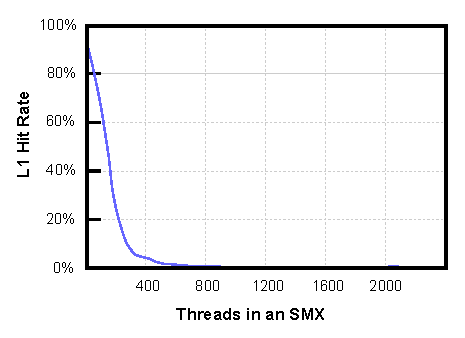
\includegraphics[scale=0.90]{WC-L1HitRate.eps}
\caption{\footnotesize\textnormal{L1 hit rate when running \texttt{wc} on Titan Black GPU with 192 cores. The target data is partitioned into $n$ chunks with each chunk assigned to a thread for processing. With effective caching, the first access of each thread results in a miss, but the subsequent 127 accesses result in cache hits. Without effective caching, these accesses result in 128 misses.}}
\label{fig:L1HitRate}
\end{figure}

Thirdly, bottlenecks on the path from L2/DRAM to GPU cores prevent scaling of memory throughput and can prevent exploitation of the full L2 and DRAM bandwidth, as we will also show in Section~\ref{GPUBehavior}.
Thus, for memory intensive applications, average memory access latencies will be significantly higher than the latency of single, isolated accesses.

The above three factors negatively affect the workloads we are targeting in a noticeable way,
as many of the big-data computations are completely memory bound and dominated by character accesses, requiring only a
trivial amount of computation between accesses.
The end result: extremely low GPU core utilization.

In this paper, we provide a detailed characterization of the behavior of GPU memory hierarchy and then propose and evaluate
an L1-level cache implemented entirely in software to address some of its issues. %we address the issues in the GPU memory hierarchy by proposing and evaluating an L1-level cache implemented entirely in software.
The software-L1 cache (S-L1) is located in software-managed GPU \emph{shared memory},
which is positioned at the same level as the L1, has the same access latency as the L1  (80 cycles on the Nvidia GTX Titan Black), and is also small (max.\ 48KB per GTX Titan Black multiprocessor).
S-L1 does not require modifications to the GPU application code; instead the compiler inserts the code required to implement S-L1.

The design of the S-L1 is guided by three key principles to deal with the small size of
the shared memory:
\begin{enumerate}
\item {\bf Private cache segments}: the S-L1 is partitioned into thread-private cache lines,
instead of having all threads share the cache space; 
\item {\bf Smaller cache lines}: the cache-line size is chosen to be 16B, which is less than the 128B that is typical in GPUs, and is thus able to serve a larger number of threads effectively;
\item {\bf Selective caching}: the S-L1 caches only the data of only those data structures where caching is most effective.
\end{enumerate}
The objective of this design is to significantly decrease average memory access times and reduce 
cache thrashing. 
It is implemented entirely in software using a fairly straightforward runtime scheme where the code
to manage and use the cache is added by using simple compiler transformations.
The specific parameters of the S-L1 cache are determined at runtime during an initial brief
monitoring phase, which also identifies the potential cache hit rate of each data structure.
After the monitoring phase, the computation is executed using the S-L1 cache for the data structures expected to have a sufficiently
high cache hit rate, given the determined amount of cache space available to each thread.

%\todo{Seems to me, we should in the following sentence first present slowdowns/speedup when compared against H-L1, and then compare it against no-L1. Reza: I'll fix it.}

In our experimental evaluation using ten GPU-local applications, S-L1 achieves an average speedup of 1.9 over hardware L1 and an average speedup of 2.1
over no L1 caching. (Compared to hardware L1, S-L1 performance ranges from a slowdown of 0.14 to a speedup of 4.3, and compared to no L1, S-L1
performance ranges from a slowdown of 0.05 to a speedup of 6.5.) These speedups are achieved despite each memory access requiring the additional
execution of at least 4 instructions (and up to potentially hundreds of instructions) when running S-L1. 
Combining S-L1 with BigKernel, the fastest known technique accelerating GPU applications processing
large data sets initially located in CPU memory~\cite{mokhtari2014bigkernel}, leads to an average speedup 1.19 over BigKernel alone,
and an average speedup of 3.7 the fastest CPU multicore implementation
of the same applications. (Compared to BigKernel alone, the speedups range from 1.04 to 1.45, and compared to the CPU implementations, the speedups range from
1.3 and 6.37.)

This paper makes the following two specific contributions:
\begin{enumerate}
\item we characterize the performance behavior of the GPU memory hierarchy and identify some of its bottlenecks using a number of experiments, and
\item we propose S-L1, a level-1 cache implemented entirely in software and evaluate its performance; novel features of S-L1 include a run-time scheme to automatically determine the parameters to configure the cache, selective caching, and thread-specific cache partitions.
\end{enumerate}

It should be noted that S-L1 is designed and effective only for a specific workload we are targeting; other workloads may well require different design parameters or not benefit from a software implementation at all.
S-L1 can be enabled/disabled on a per application basis.
While a software implementation of the L1 cache adds considerable base overhead that has to be amortized, having the implementation be in software allows easier customization.
%\todo{Good enough?  Yes.}

Our paper is organized as follows. 
Section~\ref{sec:background} describes background information about GPUs, some architectural trends we have observed over the past years, and a few micro-architectural behavior that motivated us to do this work. 
We described the design and implementation of S-L1 in Section~\ref{sec:design} and present the results of our experimental performance evaluations in Section~\ref{sec:results}.  
Section~\ref{sec:related} discusses related work, and we close with concluding remarks in 
Section~\ref{sec:conclusion}.




